\documentclass{article}
\usepackage{tbil-de}
\usepackage[top=1in,bottom=1in,right=1in,left=1in]{geometry}

\parindent=0pt

%Problem environment -- takes an argument which is the standard
\newenvironment{problem}[1]
%before
{
  \begin{flushleft}
  %{\bfseries \arabic{problem} .}
  %Problem numbering by standard
  \textbf{#1}.
  \ignorespaces
}
%after
{
  \end{flushleft}
}

\newenvironment{solution}
%before
{
  \ignorespaces
  \textbf{Solution:}
}
%after
{
  \ignorespacesafterend
  \begin{flushright}
  {\bfseries \qed}
  \end{flushright}
}



\begin{document}

\begin{center}
\Large \textbf{Sample Assessment Exercises}
\end{center}

This document contains one exercise and solution for each standard.
The goal is to give you an idea of what the exercises might look like,
and what the expectations for a complete solution are.

\begin{problem}{C1}
Sketch a solution curve through each point marked in the slope field.

\begin{center}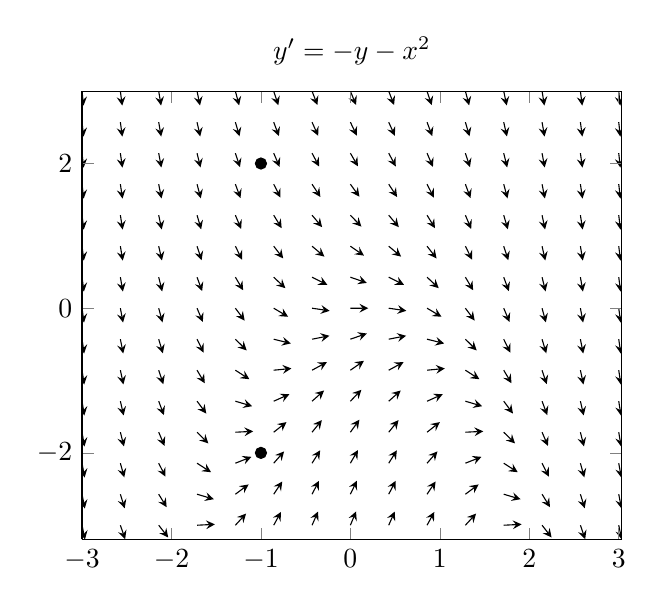
\begin{tikzpicture}
    \begin{axis}[
        title={\(y' = -y -x^2 \)},
        domain=-3:3,
        view={0}{90},
        axis background/.style={fill=white},
    ]
        \addplot3[black,
            quiver={
             u={1/(sqrt(1 + (-y -x*x)^2))},
             v={(-y - x*x)/(sqrt(1 + (-y - x*x)^2))},
             scale arrows=0.2,
            },
            -stealth,samples=15]
                {exp(-x) - 1/2*sin(x) - 1/2*cos(x)};
        %KAWWWWWWW
        % Here be some points added to the swoopy loop vector fieldamagigs
        \addplot[mark=*] coordinates {(-1,2)}; % Obvious ordered pair for lococation
        \addplot[mark=*] coordinates {(-1,-2)};
    \end{axis}
\end{tikzpicture}\end{center}
\end{problem}


\begin{solution}

\begin{center}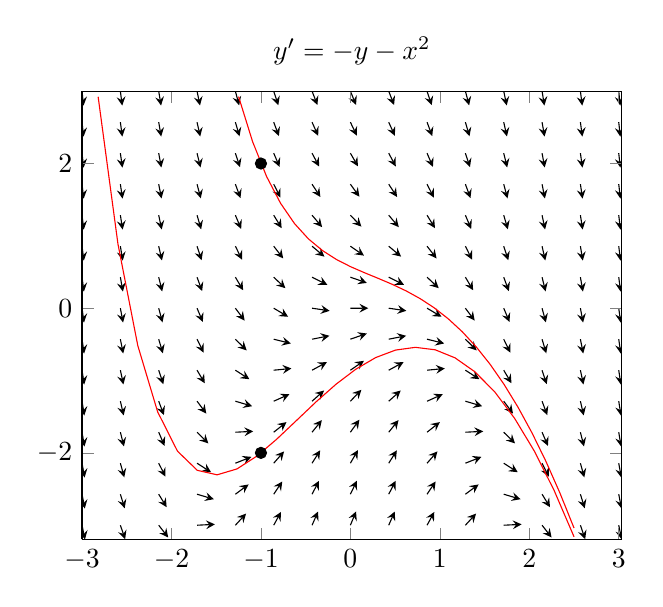
\begin{tikzpicture}
    \begin{axis}[
        title={\(y' = -y - x^2\)},
        domain=-3:3,
        view={0}{90},
        axis background/.style={fill=white},
    ]
        \addplot3[black,
            quiver={
             u={1/(sqrt(1 + (-y -x*x)^2))},
             v={(-y - x*x)/(sqrt(1 + (-y - x*x)^2))},
             scale arrows=0.2,
            },
            -stealth,samples=15]
                {exp(-x) - 1/2*sin(x) - 1/2*cos(x)};
        %KAWWWWWWW
        % Here be some points added to the swoopy loop vector fieldamagigs
        \addplot[mark=*] coordinates {(-1,2)}; % Obvious ordered pair for lococation
		\addplot[red,domain=-1.25:2.5] {-x^2+2*x-2+7/exp(1)*exp(-x)};
        \addplot[mark=*] coordinates {(-1,-2)};
		\addplot[red,domain=-2.82:2.5] {-x^2+2*x-2+3/exp(1)*exp(-x)};
    \end{axis}
\end{tikzpicture}\end{center}
\end{solution}


\begin{problem}{C2}
Find the general solution to \[y'+y=-t^2.\]
\end{problem}
\begin{solution}
First, we find a general solution to the homogeneous equation \[y'+y=0.\]  This has auxilliary equation \(r+1=0\), which has a single root at \(r=1\), so \(ce^{-t}\) is a solution.  We can find a particular solution \(y_p\) to the given equation by using undetermined coefficients; since \(-t^2\) is a polynomial, we let \(y_p = At^2+Bt+D\) and determine the coefficients \(A\), \(B\), and \(D\).  
\begin{align*}
y_p ^\prime +y_p= &= (2At+B)+(At^2+Bt+D) \\
&= At^2+(2A+B)+(B+D)
\end{align*}

So if \(y_p\) is a solution, we must have \(y_p ^\prime+y_p = -t^2\), giving us the system of equations
\begin{align*}
A&=-1 \\ 2A+B &= 0 \\ B+D&=0
\end{align*}
Thus we easily deduce that \(A=-1\), \(B=2\), and \(D=-2\), giving \(y_p = -t^2+2t-2\).  Thus, the general solution is
\[y = -t^2+2t-2+ce^{-t}.\]
\end{solution}

\begin{problem}{C3}
Find the general solution to \[y''+6y'+13y=0.\]
\end{problem}
\begin{solution}
We begin by writing the auxilliary equation \(r^2+6r+13=0\) and finding the roots.  There are many ways to do this; here, we complete  the square:
\[0=r^2+6r+13=r^2+6r+9+4=(r+3)^2+4.\]
Thus, we can easily solve to obtain \(r=-3\pm2i\).  Thus the general solution is
\[ y= c_1 e^{-3t} \cos(2t) + c_2 e^{-3t} \sin(2t) .\]
\end{solution}

\end{document}
